\chapter{Constraining {\normalfont \scshape Galacticus}}

\section{Model Accuracy}\label{sec:ModelAccuracy}

The model accuracy script processes the model described by a standard \glc\ constraints configuration file to assess how accurate the model is. Specifically, it determines the relative contribution to the covariance of each constraint arising from the finite number of merger trees run in the model and the intrinsic covariance of the observations. An accurate model should make a negligible contribution to the covariance.

To run the model accuracy script use
\begin{verbatim}
 constraints/testModelAccuracy.pl <configFile>
\end{verbatim}
where {\normalfont \ttfamily configFile} is the name of the configuration file. The script will run the model multiple times, reducing the number of trees per decade by a factor of two each time (this is done 8 times, such that the smallest model run has a factor 128 times fewer trees than the original model). Furthermore, this sequence of models is run for three different choices for sampling halo masses: {\normalfont \ttfamily powerLaw}, {\normalfont \ttfamily haloMassFunction}, and {\normalfont \ttfamily stellarMassFunction} (see \S\ref{sec:MassSamplingDensityFunction}).

For each constraint in the specified constraint compilation and accuracy measure is constructed which is the root mean squared ratio of the error arising from the finite number of trees and the intrinsic error of the constraint data. 

Accuracy analysis files are written to:
\begin{verbatim}
 <workDirectory>/accuracy
\end{verbatim}
For each constraint in the compilation a plot showing accuracy measure as a function of CPU time is written to
\begin{verbatim}
 <constraintLabel>_mergerTreeBuildTreesPerDecade.pdf
\end{verbatim}
Each point in the plot is labelled with the number of merger trees per decade. An accurate model should have accuracy measure significantly below unity. This plot is also useful to see which sampling method achieves that accuracy in the least amount of CPU time.

Additionally, a report is written to:
\begin{verbatim}
 <constraintLabel>Report.txt
\end{verbatim}
This file lists, for each sampling method, the accuracy measure achieved and the CPU time taken for the largest model run.

\section{Model Convergence}\label{sec:ModelConvergence}

The model convergence script processes the model described by a standard \glc\ constraints configuration file to assess how well converged the model is with respect to several of \glc's numerical parameters. Specifically, it determines the a covariance measure for each constraint in the specified compilation file.

To run the model convergence script use
\begin{verbatim}
 constraints/testConvergnce.pl <configFile>
\end{verbatim}
where {\normalfont \ttfamily configFile} is the name of the configuration file. The script will run the model multiple times, adjusting the value of a numerical parameter each time.

For each constraint in the specified constraint compilation a convergence measure, $C$, is constructed which
\begin{equation}
 C = \sum_i {(y_i - y_{\mathrm{ideal}, i})^2 \over \sqrt{2} \sigma_{\mathrm{ideal}, i}^2}
\end{equation}
where $y_i$ is the result of the constraint, $\sigma_i$ is the error on the result, and subscript ``ideal'' refers to the model with the most ideal value (i.e. that in the original, unmodified model) of the numerical parameter being tested (which might be the lowest value for a mass resolution, or the highest value for the maximum tree mass simulated for example). To be converged, the convergence measure should remain consistent with unity within a significant distance\footnote{``Significant distance'' here requires some judgement. Typically we would like for the model results to not change significantly as the value of a numerical parameter is adjusted by at least a factor of 2 away from the ideal value.} away from the ideal value.

Convergence analysis files are written to:
\begin{verbatim}
 <workDirectory>/convergence
\end{verbatim}
For each combination of constraint in the compilation and numerical parameter a plot showing the convergence measure as a function of the numerical parameter is created in:
\begin{verbatim}
 <constraintLabel>_<numericalParameter>.pdf
\end{verbatim}
Each point in the plot has an error bar since, due to the limited number of merger trees run, the convergence measure is not known with perfect precision. A horizontal line shows the desired convergence measure of unity.

Additionally, a report is written to:
\begin{verbatim}
 <constraintLabel>Report.txt
\end{verbatim}
This file lists, for each numerical parameter, the convergence measure and its error achieved by the ideal model. Additionally a normalized measure (the measure divided by its error) is listed. This normalized measure can be approximately interpretted as the number of $\sigma$ deviation from convergence.

\section{Model Discrepancy}\label{sec:ModelDiscrepancy}

Model discrepancy scripts process the model described by a standard \glc\ constraints configuration file to produce an output HDF5 file which describes a particular contribution to the model discrepancy. The format of these files is
\begin{verbatim}
HDF5 "discrepancy.hdf5" {
GROUP "/" {
   DATASET "additive" {
   }
   DATASET "multiplicative" {
   }
   DATASET "covariance" {
   }
}
\end{verbatim}
Each of the three datasets is optional (i.e. not all need be provided for each discrepancy). The {\normalfont \ttfamily additive} dataset gives an additive offset which will be applied to the relevant model results. The {\normalfont \ttfamily multiplicative} dataset similarly gives a multiplicative offset which will be applied to the relevant model results. Finally, the {\normalfont \ttfamily covariance} dataset gives the contribution from this discrepancy to the covariance matrix used in evaluating the model likelihood.

Discrepancy files are written to
\begin{verbatim}
 <workDirectory>/modelDiscrepancy/<discrepancyLabel>/discrepancy<constraintLabel>.hdf5
\end{verbatim}

Constraint scripts (see \S\ref{sec:ConstraintScripts}) accept a command line option {\normalfont \ttfamily --modelDiscrepancies} which specifies the path to the {\normalfont \ttfamily modelDiscrepancy} directory (i.e. {\normalfont \ttfamily <workDirectory>/modelDiscrepancy}) and will search for any relevant model discrepancy files and apply them in their calculations.

\subsection{Monte Carlo Merger Trees}

\glc\ typically uses Monte Carlo-generated merger trees when being constrained to fit data. These have the advantage that they can be generated for any cosmological parameters (necessary if the cosmological parameters are to be varied as part of the constraining process) and they can be generated uniquely for each model evaluation which avoids any bias introduced by using a fixed set of halos.

However, these Monte Carlo-generated trees may not precisely capture the properties of merger trees derived from a fully non-linear calculation of gravitational collapse (e.g. as performed by an N-body simulation). Therefore it is important to assess the model discrepancy arising from this limitation.

Model discrepancy files can be generated using:
\begin{verbatim}
 constraints/modelDiscrepancy/monteCarloTrees.pl config.xml
\end{verbatim}
where {\normalfont \ttfamily config.xml} is a standard \glc\ constraint configuration file. The script will run two sets of models, one using N-body merger trees derived from the \gls{millenniumSimulation}, and a second using Monte Carlo-generated merger trees. The number of subvolumes of the \gls{millenniumSimulation} to use is specified by the {\normalfont \ttfamily subVolumeCount} option to this script (a default of $32$ subvolumes is used if no number is specified). The subvolume data will be downloaded from the \gls{millenniumSimulation} database if necessary.

To make a fair comparison, \gls{millenniumSimulation} merger trees have their branches pruned below a mass corresponding to $20$ particles, and the Monte Carlo merger trees are built with the equivalent mass resolution. Additionally, the Monte Carlo merger trees are regridded onto a set of timesteps matched to the \gls{millenniumSimulation}.

A multiplicative model discrepancy is computed for each constraint included in the compilation (as specified in the configuration file) equal to the ratio of the N-body result to the Monte Carlo result. Additionally, the subvolumes of the \gls{millenniumSimulation} are used to estimate the covariance in the N-body result due to the finite volume of the simulation. The result is computed for each subvolume separately and the covariance of the result between subvolumes computed. This is repeated using pairs of subvolumes, quads of subvolumes, etc. If $2^n$ subvolumes were used, then the covariance measured from the result combining $2^{n-3}$ subvolumes is used to extrapolate the covariance for all $512$ subvolumes assuming that the covariance scales in inverse proportion to the number of subvolume used. Finally, the contribution of the Monte Carlo trees model to the covariance is assumed to be a diagonal matrix with elements equal to the square of the reported errors on the result of the model.

\subsection{Fixed Virial Orbits}

The orbital parameters of subhalos at the point of virial orbit crossing are usually drawn from an appropriate cosmological distribution. If instead fixed virial orbital parameters are used instead then term should be included in the model discrepancy accounting for this approximation. 

Model discrepancy files can be generated using:
\begin{verbatim}
 constraints/modelDiscrepancy/fixedVirialOrbits.pl config.xml
\end{verbatim}
where {\normalfont \ttfamily config.xml} is a standard \glc\ constraint configuration file. The script will run two models, one using fixed virial orbital parameters, and a second using variable orbital parameters using the {\normalfont \ttfamily Benson2005} method (see \S\ref{phys:virialOrbit:virialOrbitBenson2005}). A multiplicative model discrepancy is computed for each constraint included in the compilation (as specified in the configuration file) equal to the ratio of the variable orbits result to the fixed orbits result. Additionally, a model discrepancy covariance is computed. This is assumed to be a diagonal matrix with elements equal to the square of the reported errors on the results of the fixed and variable orbital parameters models.

\subsection{Jiang et al. (2008) Merger Time Scatter}

The \cite{jiang_fitting_2008} algorithm for the merging times of dark matter subhalos includes drawing times from a log-normal distribution of width $\sigma=0.4$ with median equal to their fitting function (see \S\ref{phys:satelliteMergingTimescales:satelliteMergingTimescalesJiang2008}). If instead zero scatter is used then a term should be included in the model discrepancy accounting for this approximation. 

Model discrepancy files can be generated using:
\begin{verbatim}
 constraints/modelDiscrepancy/jiang2008MergingTimeScatter.pl config.xml
\end{verbatim}
where {\normalfont \ttfamily config.xml} is a standard \glc\ constraint configuration file. The script will run two models, one using the default scatter specified by the configuration file, and a second using $\sigma=0.4$. A multiplicative model discrepancy is computed for each constraint included in the compilation (as specified in the configuration file) equal to the ratio of the $\sigma=0.4$ and default scatter results. Additionally, a model discrepancy covariance is computed. This is assumed to be a diagonal matrix with elements equal to the sum of the square of the reported errors on the result of the default scatter and $\sigma=0.4$ models.

\section{Constraints}\label{sec:ConstraintScripts}

Any constraint which can be applied to \glc\ is defined by two files, a configuration file and a likelihood script, which must be placed in {\normalfont \ttfamily constraints/constraints} and {\normalfont \ttfamily constraints/scripts} respectively. 

\subsection{Configuration File}\label{sec:ConstraintConfigFiles}

The configuration file should have the form:
\begin{verbatim}
<!-- Defines a constraint to match some data. -->                                          
<constraint>                                                                                                         
  <name>Long-form name of this constraint</name>                                                                      
  <label>shortLabelForThisConstraint</label>                                                                        
  <outputRedshift>0.07</outputRedshift>                                                                              
  <outputRedshift>1.00</outputRedshift>                                                                              
  <haloMassResolution>5.0e9</haloMassResolution>                                                                     
  <haloMassMinimum>2.0e10</haloMassMinimum>                                                                          
  <haloMassMaximum>2.0e14</haloMassMaximum>                                                                          
  <analysis>constraints/scripts/myAnalysisScript.pl</analysis>                                         
  <luminosity>
    <filter>UKIRT_K</filter>
    <redshift>0.0</redshift>
    <frame>rest</frame>
  </luminosity>
  <luminosity>
    <filter>UKIRT_K</filter>
    <redshift>1.0</redshift>
    <frame>observed</frame>
  </luminosity>
  <optionOn>outputMainBranchStatus</optionOn>
  <optionOn>outputDensityContrastData</optionOn>
  <parameter>
   <name>outputDensityContrastValues</name>
   <value>200.0</value>
   <accumulation>unique</accumulation>
  </parameter>
</constraint>                                                                                                        
\end{verbatim}
The {\normalfont \ttfamily name} and {\normalfont \ttfamily label} are used to describe the constraint ({\normalfont \ttfamily label} is used as a suffix in file names so should not contain spaces or other characters which might cause problems in file names). 

The remaining elements describe the requirements for this constraint. {\normalfont \ttfamily haloMassResolution} specifies the maximum resolution in mergers trees that still allows this constraint to be computed accurately. Similarly, {\normalfont \ttfamily haloMassMinimum} and {\normalfont \ttfamily haloMassMaximum} specify the required range of halo masses to simulate to allow this constraint to be computed accurately.

One or more {\normalfont \ttfamily outputRedshift} elements may be present, each specifying a redshift at which output is required for this constraint. Similarly, one or more {\normalfont \ttfamily luminosity} elements may be present, each of which specifies a luminosity which must be computed for this constraint. Each {\normalfont \ttfamily luminosity} must contain a specification of {\normalfont \ttfamily filter}, {\normalfont \ttfamily redshift}, and {\normalfont \ttfamily frame} to define which luminosity is to be computed.

One or more {\normalfont \ttfamily optionOn} elements may be present. Each element must specify the name of a \glc\ input parameter. That parameter will be set to {\normalfont \ttfamily true} in the \glc\ input parameter file.

Finally, arbitrary other parameter may be set using the standard {\normalfont \ttfamily parameter} element which should give the {\normalfont \ttfamily name} and {\normalfont \ttfamily value} for the parameter. Optionally, an {\normalfont \ttfamily accumulation} element may also be specified for each {\normalfont \ttfamily parameter}. This controls how values of the parameter are to be accumulated if set by more than one constraint. An accumulation of {\normalfont \ttfamily overwrite} will simply overwrite any previously set values. An accumulation of {\normalfont \ttfamily combine} will concatenate all values set by different constraints. Finally, an accumulation of {\normalfont \ttfamily unique} will concatenate all values set by different constraints and then filter out any duplicates.

When multiple constraints are used, their requirements are automatically combined.

\subsection{Likelihood Script}

The likelihood script for a constraint is required to perform several tasks, controlled by command line options. The script should accept the following command line syntax:
\begin{verbatim}
 myScript.pl <galacticusFile> [options...]
\end{verbatim}
where {\normalfont \ttfamily galacticusFile} is the file name of the \glc\ model for which the likelihood calculation should be performed. The following options must be supported by the script:
\begin{description}
 \item [{\normalfont \ttfamily --plotFile <fileName>}] If this option is present, the script should generate a plot showing the constraint and the model result and write it to {\normalfont \ttfamily fileName}.
 \item [{\normalfont \ttfamily --outputFile <fileName>}] If this option is present, the script should compute the log-likelihood of the model given the constraint and write it to {\normalfont \ttfamily fileName} using the format
\begin{verbatim}
 <constraint>
  <logLikelihood>-123</logLikelihood>
 </constraint>
\end{verbatim}
 \item [{\normalfont \ttfamily --accuracyFile <fileName>}] If this option is present, the script should write an XML file giving details of the accuracy of the model results relative to the observational errors using the format
\begin{verbatim}
 <accuracy>
  <x>...</x>
  .
  .
  .
  <x>...</x>
  <yModel>...</yModel>
  .
  .
  .
  <yModel>...</yModel>
  <yData>...</yData>
  .
  .
  .
  <yData>...</yData>
  <errorModel>...</errorModel>
  .
  .
  .
  <errorModel>...</errorModel>
  <errorData>...</errorData>
  .
  .
  .
  <errorData>...</errorData>
 </accuracy>
\end{verbatim}
In this file the {\normalfont \ttfamily yModel} and {\normalfont \ttfamily yData} elements should give the values of the model result and the comparable data respectively, while {\normalfont \ttfamily errorModel} and {\normalfont \ttfamily errorData} should give an estimate of the errors on these quantities. In the case of the model error this should include only the contribution arising from the finite number of merger trees simulated. This file will be used to judge whether the model is running sufficient merger trees such that the likelihood is not dominated by these errors. The {\normalfont \ttfamily x} elements are optional but can be used to give the parameter values associated with each model result.
 \item [{\normalfont \ttfamily --resultFile <fileName>}] If this option is present, the script should write an XML file giving details of the result of the model using the format
\begin{verbatim}
 <accuracy>
  <x>...</x>
  .
  .
  .
  <x>...</x>
  <y>...</y>
  .
  .
  .
  <y>...</y>
  <error>...</error>
  .
  .
  .
  <error>...</error>
 </accuracy>
\end{verbatim}
In this file the {\normalfont \ttfamily y} elements should give the values of the model result, while the {\normalfont \ttfamily error} elements should give an estimate of the errors on these results. The error should include only the contribution arising from the finite number of merger trees simulated. This file will be used to judge whether the model result is converged with respect to various numerical parameters in \glc. The {\normalfont \ttfamily x} elements are optional but can be used to give the parameter values associated with each model result.
 \item [{\normalfont \ttfamily --modelDiscrepancies <path>}] If this option is present, the script should scan {\normalfont \ttfamily path}. For each directory found in {\normalfont \ttfamily path} the script should check for the existance of a file named {\normalfont \ttfamily discrepancy<label>.hdf5} where {\normalfont \ttfamily label} is the label given for this constraint in its configuration file (see \S\ref{sec:ConstraintConfigFiles}). If present, the model discrepancy given in that file should be applied to the likelihood calculation. See \S\ref{sec:ModelDiscrepancy} for a description of the structure of the discrepancy files.
\end{description}

\subsection{Available Constraints}

\subsubsection{Caputi et al. (2011) UKIDSS UDS Stellar Mass Function}\label{sec:ConstraintsUKIDSSUDSStellarMassFunction}

The incompleteness of the observational sample (which is required when estimating the Poisson contribution to the covariance matrix) is found from the 50\% and 80\% completeness masses, $M_{50}$ and $M_{80}$ respectively, given in Fig.~4 of \cite{caputi_stellar_2011}. Specifically, we assume that, at a given mass $M$, the number of photons being received from a galaxy can be modeled as a Gaussian distribution with mean $f M$ and variance $fM+\mu$, where $\mu$ is the number of photons ariving from the sky. The fraction of sources of mass $M$ that will be detected at more than $n \sigma$ above the background is then
\begin{eqnarray}
f(M) & = & \int_{n\sqrt{mu}}^\infty {1 \over \sqrt{2 \pi} \sqrt{f M + \mu}} \exp\left( - {[S-fM]^2 \over 2 [f M + \mu]} \right) \mathrm{d}S \nonumber \\
     & = & {1 \over 2}\left[ 1 - \hbox{erf}\left( {x(M) \over \sqrt{2}} \right)  \right],
\label{eq:incompleteness}
\end{eqnarray}
where $x(M) = (n \sqrt{mu} - f M)/(\mu+fM)^{1/2}$. Given $f(M_\mathrm{50})=0.5$ and $f(M_\mathrm{80})=0.8$ we can solve for $f$ and $\mu$, and then compute the completeness in each mass using eqn.~(\ref{eq:incompleteness}). The resulting completeness curves are shown in Fig.~\ref{fig:UKIDSSUDSCompleteness}. Note that the model of eqn.~(\ref{eq:incompleteness}) is clearly an oversimplification, but should capture the expected behavior of the completeness and, since it is fit to the 50\% and 80\% completenesses reported by \cite{caputi_stellar_2011}---which were computed using detailed simulations---should work sufficiently well.

\begin{figure}
 \begin{center}
 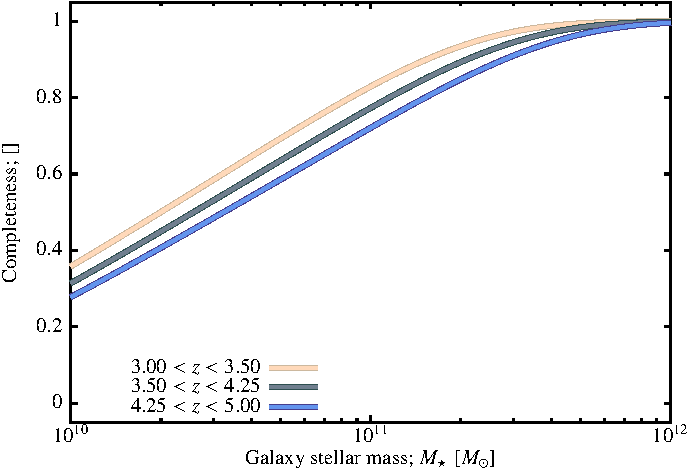
\includegraphics[width=85mm,trim=0mm 0mm 0mm 4mm,clip]{Plots/DataAnalysis/UKIDSSUDSCompleteness.pdf}
 \caption{The completeness as a function of stellar mass in the survey of \protect\cite{caputi_stellar_2011}. Curves are computed using eqn.~(\protect\ref{eq:incompleteness}) with parameters fit to the reported 50\% and 80\% completeness masses from \protect\cite{caputi_stellar_2011}.}
 \end{center}
 \label{fig:UKIDSSUDSCompleteness}
\end{figure}

\subsubsection{Bernardi et al. (2013) SDSS Stellar Mass Function}\label{sec:AnalysisBernardiSDSSStellarMassFunction}

When computing the Poisson term in the covariance matrix, the number of galaxies per bin is determined directly from the mass function, assuming a 91\% completeness\footnote{7\% arising from fiber collisions, 2\% from failures in the Pymorph pipeline (M.~Bernardi, private communication).}. The survey geometry and depth is described in \S\ref{phys:surveyGeometry:surveyGeometryBernardi2013SDSS}.

\subsubsection{Baldry et al. (2012) GAMA Stellar Mass Function}\label{sec:AnalysisBaldryGAMAStellarMassFunction}

When computing the Poisson term in the covariance matrix, the number of galaxies per bin is taken from data supplied by I.~Baldry (private communication). The survey geometry and depth is described in \S\ref{phys:surveyGeometry:surveyGeometryBaldry2012GAMA}.

Finally, the completeness of the observational sample is estimated to be greater than 98\% (P.~Norberg, private communication). Therefore we add an additional contribution to the observed covariance matrix equal to $\mathcal{C}_{ij} = 0.02 \phi_i \phi_j$ where $\phi$ is the observed mass function.

\subsubsection{Tomczak et al. (2014) ZFOURGE Stellar Mass Functions}\label{sec:AnalysisTomczakZFOURGEStellarMassFunction}

When computing the Poisson term in the covariance matrix, the number of galaxies per bin is taken directly from tables provided by R.~Quadri (private communication).

\subsubsection{Davidzon et al. (2013) VIPERS Stellar Mass Functions}\label{sec:AnalysisDavidzonVIPERSStellarMassFunction}

When computing the Poisson term in the covariance matrix, the number of galaxies per bin is taken directly from tables supplied by I.~Davidzon (private communication).

\subsubsection{Muzzin et al. (2013) ULTRAVISTA Stellar Mass Functions}\label{sec:AnalysisMuzzinULTRAVISTAStellarMassFunction}

When computing the Poisson term in the covariance matrix, the completeness is taken to be 95\% in the lowest mass bins, and 100\% in all other bins \citep{muzzin_evolution_2013}.

\subsubsection{Moustakas et al. (2013) PRIMUS Stellar Mass Functions}\label{sec:AnalysisMoustakasPRIMUSSStellarMassFunctions}

When computing the Poisson term in the covariance matrix, the number of galaxies per bin is taken directly from \cite{moustakas_primus:_2013}. The survey geometry and depth is described in \S\ref{phys:surveyGeometry:surveyGeometryMoustakas2013PRIMUS}.

\subsubsection{Martin et al. (2010) ALFALFA HI Mass Function}\label{sec:AnalysisALFALFAHIMassFunction}

When computing the Poisson term in the covariance matrix, the number of galaxies per bin is taken directly from Fig.~5 of \cite{martin_arecibo_2010} such that incompleteness is automatically accounted for. The survey geometry and depth is described in \S\ref{phys:surveyGeometry:surveyGeometryMartin2010ALFALFA}.

The resulting maximum likelihood mass function is shown in Fig.~\ref{fig:MaximumLikelihoodMassFunctionHOD}, clearly illustrating that this parametric \gls{hod} can produce an excellent match to the observed mass function. The resulting correlation matrix is shown in Fig.~\ref{fig:CorrelationMatrixALFALFA}. As expected, at the higher masses the correlation matrix is dominated by the on-diagonal terms---arising from the Poisson fluctuations in the number of galaxies due to the scarcity of these massive systems. At lower masses the matrix has significant off-diagonal amplitude, indicating strong correlations between nearby bins, arising from both large-scale structure and halo contributions to the covariance. This structure significantly weakens the constraint arising from the low-mass end of the mass function.

\begin{figure}
 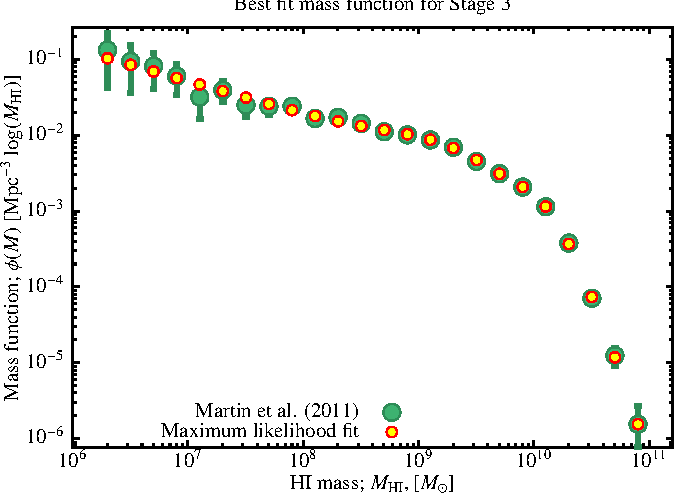
\includegraphics[width=85mm,trim=0mm 0mm 0mm 2.5mm,clip]{Plots/DataAnalysis/alfalfaHIMassFunctionBestFit.pdf}
 \caption{The maximum likelihood mass function obtained from our parametric \protect\gls{hod} (yellow points), compared to the observed HI mass function of \protect\citeauthor{martin_arecibo_2010}~(\citeyear{martin_arecibo_2010}; green points).}
 \label{fig:MaximumLikelihoodMassFunctionHOD}
\end{figure}

\begin{figure}
 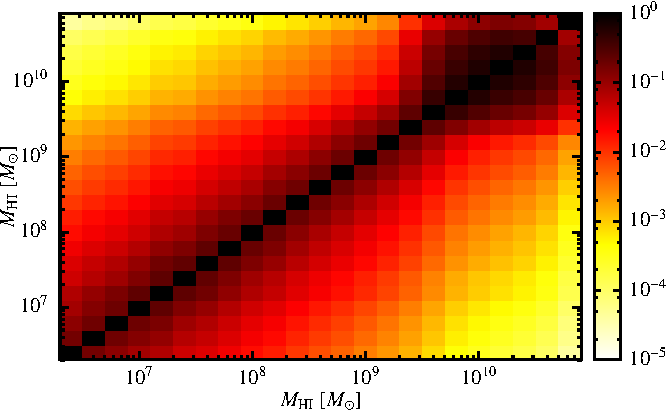
\includegraphics[width=85mm,trim=0mm 0mm 0mm 0mm,clip]{Plots/DataAnalysis/alfalfaHICorrelationmatrix.pdf}
 \caption{The correlation matrix of the observed galaxy HI mass function of \protect\cite{martin_arecibo_2010}. Color indicates the strength of correlation between bins, according to the scale shown on the right.}
 \label{fig:CorrelationMatrixALFALFA}
\end{figure}

\subsubsection{Shen et al. (2003) Late-Type Galaxy Size Distribution}\label{sec:SDSSLateTypeGalaxySizeDistribution}

The covariance matrix is computed as
\begin{equation}
 \mathbf{C} = \mathbf{C}_\mathrm{obs} + \mathbf{C}_\mathrm{model,random} + \sum_i \mathbf{C}_{\mathrm{discrepancy}, i},
\end{equation}
where $\mathbf{C}_\mathrm{obs}$ is the covariance matrix of the observational data, $\mathbf{C}_\mathrm{model,random}$ is the covariance matrix of the model arising from random noise (due to the finite number of trees simulated, and $\mathbf{C}_{\mathrm{discrepancy}, i}$ is the covariance due to the $i^\mathrm{th}$ model discrepancy.

The model covariance matrix is estimated using the sample methods as described in \S\ref{sec:AnalysisALFALFAHIMassFunction}. The only difference is that in this case we have a 2-D histogram. This 2-D histogram is ``flattened'' into a 1-D vector for purposes of likelihood computation however, so covariance matrix estimation proceeds unchanged. (Note that correlations between mass bins are accounted for, in additional to correlations between radius bins.) Since the radius functions of \cite{shen_size_2003} are normalized to unity at each mass, we must account for this in the covariance matrix. The radius function transforms as:
\begin{equation}
 f_{ik} \rightarrow {f_{ik} \over \Delta \log_{10} R \sum_i f_{ik} },
\end{equation}
where $i$ indexes radius bins, $k$ indexes mass bins, and $\Delta \log_{10} R$ is the width of the radius bin. The Jacobian of this transformation is simply
\begin{equation}
 J_{ij} = {\delta_{ij} - f_i \over  \Delta \log_{10} R \sum_i f_{ik}}.
\end{equation}
Therefore, the covariance matrix is modified according to $\mathcal{C} \rightarrow J \mathcal{C} J^\mathrm{T}$. The same transformation is applied to the covariance matrix of the observed data (for which the reported errors are simply the Poisson errors on each bin).

The model likelihood is then computed using:
\begin{equation}
 \mathcal{L} = {1 \over \sqrt{(2 \pi)^n |\mathbf{C}|}} \exp\left[ -{1\over 2} \Delta \mathbf{C}^{-1} \Delta \right],
\end{equation}
where $\Delta_i = \Phi_{\mathrm{model}, i} - \Phi_{\mathrm{observed}, i}$ is the difference between the model and observed mass functions, and $n$ is the number of points in the mass function histogram.

\section{Constraint Compilations}

To specify which constraints will be applied to a particular model, a compilation file is used. These must be stored in {\normalfont \ttfamily constraints/compilations}. An example of such a file follows:
\begin{verbatim}
<constraintCompilation>
  <constraint>
    <definition>constraints/constraints/stellarMassFunction_SDSS_z0.07.xml</definition>
    <weight>1.0</weight>
  </constraint>
  <constraint>
    <definition>constraints/constraints/hiMassFunction_ALFALFA_z0.00.xml</definition>
    <weight>1.0</weight>
  </constraint>
</constraintCompilation>
\end{verbatim}
Each {\normalfont \ttfamily constraint} element specifies one constraint that will be included in this compilation, and must contain a {\normalfont \ttfamily definition} element, giving the path of the configuration file for this constraint, and a {\normalfont \ttfamily weight} element which allows the relative weight given to each constraint to be varied\footnote{Note that, if your constraints are computing correct likelihoods, re-weighting them may not be a good idea. \emph{Caveat constrainor.}}.

\section{Constraint File}

\glc\ has a complete constraints infrastructure which implements various \gls{mcmc} algorithms to analyze the posterior probability distribution of the model given some compilation of constraints. The infrastructure is \gls{mpi} parallelized and ideal for running on large compute clusters.

To perform a constraint calculation simply build the constraint code:
\begin{verbatim}
 make Constrain_Galacticus.exe
\end{verbatim}
and run with a parameter file and configuration file. Typically, you will want to run this code under \gls{mpi}, for example:
\begin{verbatim}
 mpirun -n 4 Constrain_Galacticus.exe mcmcParameters.xml mcmcConfig.xml
\end{verbatim}
would run 4 processes (typically you will need to run many more than this). If running on a \gls{pbs} queue, embed this command in a suitable \gls{pbs} script and submit. 

The parameter file follows the same format as a standard \glc\ parameter file and specifies the values of parameters to be used. For example, the seed used fo pseudo-random number sequences can be specified in this file. 

The configuration file specifies the details of the constraint simulation to be performed. An example configuration file is:
\begin{verbatim}
<?xml version="1.0" encoding="UTF-8"?>
<simulationConfig>

  <likelihood>
    <type>Galacticus</type>
    <name>verySimplisticToStellarMassFunction</name>
    <compilation>stellarMassFunction_SDSS_z0.07.xml</compilation>
    <baseParameters>./mcmcWork/verySimplisticToStellarMassFunctionBase.xml</baseParameters>
    <workDirectory>./mcmcWork</workDirectory>
    <scratchDirectory>./mcmcScratch</scratchDirectory>
    <report>no</report>
    <randomize>no</randomize>
    <threads>4</threads>
    <saveState>no</saveState>
    <cpulimit>1200</cpulimit>
    <coredump>NO</coredump>
    <coredumpsize>0</coredumpsize>
    <sequentialModels>no</sequentialModels>
    <memoryLimit>2gb</memoryLimit>
    <environment>LD_LIBRARY_PATH=/opt/gcc-trunk/lib:/opt/gcc-trunk/lib64:/usr/local/upstream/lib:$LD_LIBRARY_PATH</environment>
    <environment>PATH=/opt/gcc-trunk/bin:$PATH</environment>
  </likelihood>

  <convergence>
    <type>GelmanRubin</type>
    <Rhat>1.2</Rhat>
    <burnCount>100</burnCount>
    <testCount>100</testCount>
    <outlierCountMaximum>0</outlierCountMaximum>
    <outlierSignificance>0.95</outlierSignificance>
    <outlierLogLikelihoodOffset>60</outlierLogLikelihoodOffset>
  </convergence>
  
  <state>
    <type>history</type>
    <acceptedStateCount>100</acceptedStateCount>
  </state>
  
  <proposalSize>
    <type>adaptive</type>
    <gammaInitial>1.77</gammaInitial>
    <gammaFactor>1.414</gammaFactor>
    <acceptanceRateMinimum>0.4</acceptanceRateMinimum>
    <acceptanceRateMaximum>0.6</acceptanceRateMaximum>
    <updateCount>10</updateCount>
  </proposalSize>
  
  <randomJump>
    <type>adaptive</type>
  </randomJump>
  
  <simulation>
    <type>temperedDifferentialEvolution</type>
    <stepsMaximum>1000000</stepsMaximum>
    <stepsPostConvergence>100000</stepsPostConvergence>
    <acceptanceAverageCount>100</acceptanceAverageCount>
    <logFileRoot>./mcmcWork/mcmc/chains</logFileRoot>
    <temperatureMaximum>64.0</temperatureMaximum>
    <untemperedStepCount>20</untemperedStepCount>
    <temperedLevels>10</temperedLevels>
    <stepsPerLevel>10</stepsPerLevel>
    <logFlushCount>10<logFlushCount>
  </simulation>

  <parameters>
    <parameter>
      <name>starFormationTimescaleDisksHaloScalingVirialVelocityExponent</name>
      <prior>
	<distribution>
	  <type>uniform</type>
	  <minimum>-6.0</minimum>
	  <maximum>+0.0</maximum>
	</distribution>
      </prior>
      <mapping>
        <type>linear</type>
      </mapping>
      <random>
	<type>Cauchy</type>
	<median>0.0</median>
	<scale>0.006</scale>
      </random>
    </parameter>
    <parameter>
      <name>starFormationTimescaleDisksHaloScalingRedshiftExponent</name>
      <prior>
	<distribution>
	  <type>uniform</type>
	  <minimum>-1.0</minimum>
	  <maximum>+4.0</maximum>
	</distribution> 
      </prior>
      <mapping>
        <type>linear</type>
      </mapping>
      <random>
	<type>Cauchy</type>
	<median>0.0</median>
	<scale>0.005</scale>
      </random>
    </parameter>
  </parameters>
  
</simulationConfig>
\end{verbatim}

\subsection{Parameters and Priors}\label{sec:ParametersPriors}

The {\normalfont \ttfamily parameters} section contains a list of all parameters to be varied in the analysis. Each parameter is described by one {\normalfont \ttfamily parameter} element. That element must contain a {\normalfont \ttfamily name} element, which gives the name of the parameter, a {\normalfont \ttfamily prior} element that contains a {\normalfont \ttfamily distribution} element defining the distribution for this prior, a {\normalfont \ttfamily mapping} element that describes the mapping of the parameter into the internal state used in \gls{mcmc} calculations, and (for differential evolution simulations) a {\normalfont \ttfamily random} element that defines the distribution to be used for the random perturbation to be added to this parameter in proposals.

The {\normalfont \ttfamily name} element can specify subparameters, elements in an array of parameters, and elements within a parameter's {\normalfont \ttfamily value} element. For example, consider the parameter file:
\begin{verbatim}
<parameter1 value="123"/>
<parameterA value="456"/>
<parameterA value="789"/>
<parameterA value="987"/>
<parameter2 value="abc">
 <parameter2a value="def"/>
</parameter2>
<parameterX value="1.0 2.0 3.0"/>
\end{verbatim}
\begin{itemize}
\item A name of {\normalfont \ttfamily parameter1} will change the value ({\normalfont \ttfamily 123}) of the {\normalfont \ttfamily parameter1} element;
\item A name of {\normalfont \ttfamily parameterA[1]} will change the value ({\normalfont \ttfamily 1789}) of the second {\normalfont \ttfamily parameterA} element (array indexing is 0-offset);
\item A name of {\normalfont \ttfamily parameter2->parameter2a} will change the value ({\normalfont \ttfamily def}) of the {\normalfont \ttfamily parameter2a} element;
\item A name of {\normalfont \ttfamily parameterX{1}} will change the value ({\normalfont \ttfamily 2.0}) of second entry in the value of the {\normalfont \ttfamily parameterX} element.
\end{itemize}

Currently allowed mappings are:
\begin{itemize}
\item[{\normalfont \ttfamily linear}] Effectively a null mapping, as the parameter is mapped into itself: $x \rightarrow x$.
\item[{\normalfont \ttfamily logarithmic}] The parameter is mapped logarithmically: $x \rightarrow \log(x)$. This mapping can be applied only to uniform priors.
\end{itemize}
Note that the mapping will map the values of the prior. For example, if you specify a uniform prior with a logarithmic mapping, the upper and lower limits of the prior should be specified on $x$, not on $\log(x)$. These limits will be mapped appropriately internally.

\subsubsection{Loading External Parameters/Priors}

It is also possible to load parameters and their priors from external files. This is useful to add common sets of parameters, such as cosmological parameter. To do so, add an element of the form:
\begin{verbatim}
<xi:include href="../../constraints/parameters/wmap9Cosmology.xml" 
   xmlns:xi="http://www.w3.org/2001/XInclude" />
\end{verbatim}
\emph{after} the {\normalfont \ttfamily parameters} section of the constraint file. The {\normalfont \ttfamily href} attribute must give the path (relative to the constraint file, or absolute) to the external parameter file. This file should contain its own {\normalfont \ttfamily parameters} block, describing all parameters to be varied along with their priors. 

\subsubsection{Derived Parameter Values}

It is possible to define parameters in terms of other parameters. Common uses for this include:
\begin{itemize}
 \item Setting $\Omega_\Lambda$ from the value of $\Omega_\mathrm{M}$ to enforce a flat Universe;
 \item Setting the values of parameters with correlated priors as linear combinations of dummy parameters for which the priors are independent.
\end{itemize}
To define a parameter in this way include a {\normalfont \ttfamily parameter} element of the form:
\begin{verbatim}
<parameter>
 <name>sigma_8</name>
 <define>0.8178+%cosmology0*0.003817+%cosmology1*0.007931+%cosmology2*0.01002
    +%cosmology3*0.001584+%cosmology4*0.002931+%cosmology5*0.001727</define>
</parameter>
\end{verbatim}
Here the {\normalfont \ttfamily define} element gives an equation for the parameter in terms of other parameters. All standard mathematical operators and functions (as recognized by Perl) can be used, and other parameters referenced by using their name prefixed with a ``\%''.

\subsubsection{Including External Parameters}

Predefined sets of parameters (along with their priors) can be included using the {\normalfont \ttfamily xi:include} element. For example,
\begin{verbatim}
 <xi:include href="../../constraints/parameters/wmap7Cosmology.xml"
    xmlns:xi="http://www.w3.org/2001/XInclude" />
\end{verbatim}
will include a set of parameters from the file {\normalfont \ttfamily ../../constraints/parameters/wmap7Cosmology.xml} which defines priors on cosmological parameters consistent with the covariance matrix of the WMAP-7 cosmological constraints \citep{komatsu_seven-year_2010}.
